\documentclass[ 12pt ]{article}

\usepackage{amsmath}
\usepackage{amssymb}
\usepackage{cancel}
\usepackage{tikz}
\usepackage{listings}
\usepackage{mathdots}
\usepackage[margin=.75in]{geometry}

\usetikzlibrary{arrows}

\tikzset{
  treenode/.style = {align=center, inner sep=0pt, text centered,
    font=\sffamily},
  arn_n/.style = {treenode, circle, white, font=\sffamily\bfseries, draw=black,
    fill=black, text width=1.5em},%
  arn_r/.style = {treenode, circle, red, draw=red, 
    text width=1.5em, very thick},%
  arn_x/.style = {treenode, rectangle, draw=black,
    minimum width=0.5em, minimum height=0.5em},%
  arn_p/.style = {treenode, circle, white, font=\sffamily\bfseries, draw=black,
    fill=purple, text width=1.5em},%
}

\begin{document}

% title page
\title{%
	Homework 5 \\
	\large CS 477 Analysis of Algorithims \\
	Section 1001}
\author{Landon Fox}
\date{March 10, 2020}
\maketitle
\newpage

\begin{itemize}
	% problem 1
	\item[] {1) \large}
	\begin{itemize}
		% problem 1a
		\item[] 1a)
		\begin{flalign}
			E[X] &= 2P\{X=H\} - 1P\{X=T\} \nonumber \\
			&= 2 \cdot \frac{3}{4} - 1 \cdot \frac{1}{4} \nonumber \\
			&= \frac{5}{4} \nonumber
		\end{flalign}

		% problem 1b
		\item[] 1b)
		\begin{flalign}
			E[X] &= 10P\{X=Red\} + 5P\{X=Yellow\} + 2P\{X=Blue\} + 1P\{X=Green\} + 0 \nonumber \\
			&= 10 \cdot \frac{1}{10} + 5 \cdot \frac{3}{20} + 2 \cdot \frac{1}{5} + 1 \cdot \frac{1}{4} \nonumber \\
			&= \frac{12}{5} \nonumber
		\end{flalign}
	\end{itemize}

	% problem 2
	\item[] {2) \large}
	$i$ starts at $\left \lfloor \frac{n}{2} \right \rfloor$ which represents the last element in the heap that is not a leaf. 
	It counts down to one rather than up because calling $max\_heapify$ requires that the child nodes of the given subtree must also be heaps.
	By starting at the bottom and heading to the root, you can guarantee all child nodes are heaps. Otherwise the same cannot be said.

	% problem 3
	\item[] {3) \large}
	\begin{itemize}
		% problem 3a
		\item[] 3a)
		\begin{center}
			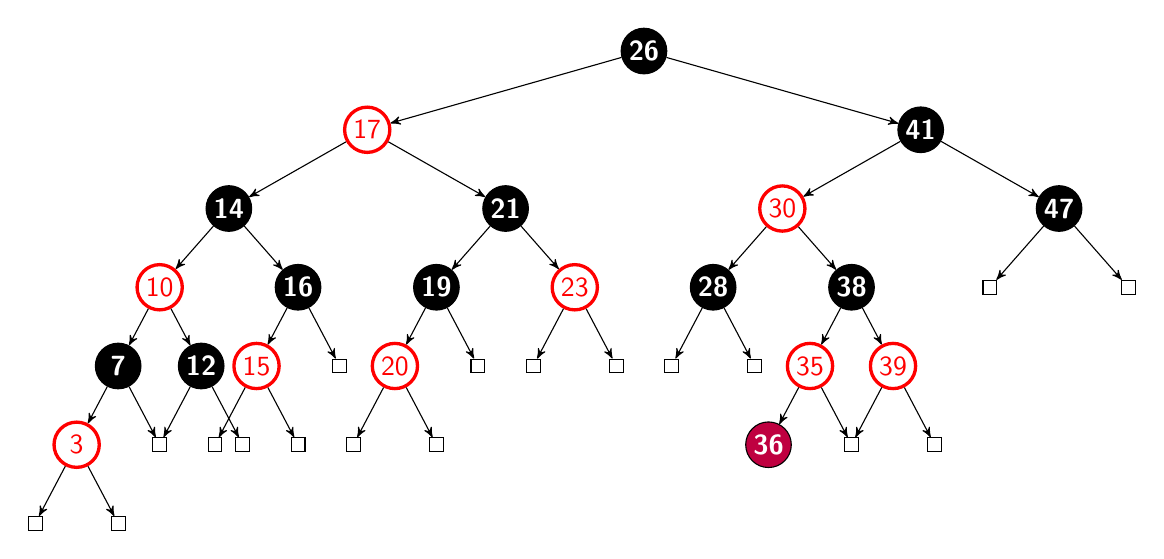
\begin{tikzpicture}[->,>=stealth',
				level 1/.style={sibling distance=20em},
			  	level 2/.style={sibling distance=10em},
			  	level 3/.style={sibling distance=5em},
			  	level 4/.style={sibling distance=3em},
			  	level 5/.style={sibling distance=3em},
			  	level 6/.style={sibling distance=3em},
				level/.style={ level distance = 1cm}] 
				\node [arn_n] {26}
				    child { node [arn_r] {17}
						child { node [arn_n] {14}
							child { node [arn_r] {10}
								child { node [arn_n] {7}
									child { node [arn_r] {3}
										child { node [arn_x] {} }
										child { node [arn_x] {} }
									}
									child { node [arn_x] {} }
								}
								child { node [arn_n] {12}
									child { node [arn_x] {} }
									child { node [arn_x] {} }
								}
							}
							child { node [arn_n] {16}
								child { node [arn_r] {15}
									child { node [arn_x] {} }
									child { node [arn_x] {} }
								}
								child { node [arn_x] {} }
							}
						}
						child { node [arn_n] {21}
							child { node [arn_n] {19}
								child { node [arn_r] {20}
									child { node [arn_x] {} }
									child { node [arn_x] {} }
								}
								child { node [arn_x] {} }
							}
							child { node [arn_r] {23}
								child { node [arn_x] {} }
								child { node [arn_x] {} }
							}
						}
					}
					child { node [arn_n] {41}
						child { node [arn_r] {30}
							child { node [arn_n] {28}
								child { node [arn_x] {} }
								child { node [arn_x] {} }
							}
							child { node [arn_n] {38}
								child { node [arn_r] {35}
									child { node [arn_p] {36} }
									child { node [arn_x] {} }
								}
								child { node [arn_r] {39}
									child { node [arn_x] {} }
									child { node [arn_x] {} }
								}
							}
						}
						child { node [arn_n] {47}
							child { node [arn_x] {} }
							child { node [arn_x] {} }
						}
					};
			\end{tikzpicture}
		\end{center}
		If node $36$ is red, the resulting tree is not a red-black tree. A red node cannot have a red child. Violation of axiom $4$. \\ \\
		If node $36$ is black, the resulting tree is not a red-black tree. The respective path from the root to the leaf does not have the same black height
		as all other paths. Violation of axiom $5$.

		% problem 3b
		\item[] 3b)
		Yes it would be a red-black tree. No axioms are violated. If the tree originally had a red node, its immediate children must be black so axiom $4$ is not violated.
		Similarly, axiom $5$ is not threatened because we don't account for the root's color in accounting for black height.
	\end{itemize}

	% problem 4
	\item[] {4) \large}
	The black height is the shortest path possible from a node to a leaf. That means that the longest path may have a red node in between each black node, therefore
	giving a height twice the shortest path.
	\begin{flalign}
		height(x) \leq 2 \cdot black\_height(x) \nonumber
	\end{flalign}

	% problem 5
	\item[] {5) \large}
	\begin{flalign}
		let\;\;\; &x:\; number\; of\; 2s \nonumber \\
		&y:\; number\; of\; 7s \nonumber
	\end{flalign}
	\begin{flalign}
		know\;\;\; 12 &= x + y \nonumber \\
		E[X] &= 3.25 \nonumber
	\end{flalign}
	\begin{flalign}
		E[X] &= 2P\{X=2\} + 7P\{X=7\} \nonumber \\
		3.25 &= 2 \cdot \frac{x}{x+y} + 7 \cdot \frac{y}{x+y} \nonumber \\
		\frac{13}{4}(x+y) &= 2x + 7y \nonumber \\
		x &= 3y \nonumber \\
		Substitution:\;\;\; 3y+y &= 12 \nonumber \\
		y &= 3 \nonumber \\
		x &= 3 \cdot 3 \nonumber \\
		x &= 9 \nonumber
	\end{flalign}

	% problem 6
	\item[] {6) \large}
	\begin{flalign}
		P\{X=x_1\} &= P\{X=x_2\} = \hdots = P\{X=x_n\} = \frac{1}{n} \nonumber \\
		E[X] &= x_1 \cdot \frac{1}{n} + x_2 \cdot \frac{1}{n} + \hdots + x_n \cdot \frac{1}{n} \nonumber \\
		&= \frac{x_1 + x_2 + x_3 + \hdots + x_n}{n} = \overline{x} \nonumber
	\end{flalign}
\end{itemize}

\end{document}
